
% Default to the notebook output style

    


% Inherit from the specified cell style.




    
\documentclass[11pt]{article}

    
    
    \usepackage[T1]{fontenc}
    % Nicer default font (+ math font) than Computer Modern for most use cases
    \usepackage{mathpazo}

    % Basic figure setup, for now with no caption control since it's done
    % automatically by Pandoc (which extracts ![](path) syntax from Markdown).
    \usepackage{graphicx}
    % We will generate all images so they have a width \maxwidth. This means
    % that they will get their normal width if they fit onto the page, but
    % are scaled down if they would overflow the margins.
    \makeatletter
    \def\maxwidth{\ifdim\Gin@nat@width>\linewidth\linewidth
    \else\Gin@nat@width\fi}
    \makeatother
    \let\Oldincludegraphics\includegraphics
    % Set max figure width to be 80% of text width, for now hardcoded.
    \renewcommand{\includegraphics}[1]{\Oldincludegraphics[width=.8\maxwidth]{#1}}
    % Ensure that by default, figures have no caption (until we provide a
    % proper Figure object with a Caption API and a way to capture that
    % in the conversion process - todo).
    \usepackage{caption}
    \DeclareCaptionLabelFormat{nolabel}{}
    \captionsetup{labelformat=nolabel}

    \usepackage{adjustbox} % Used to constrain images to a maximum size 
    \usepackage{xcolor} % Allow colors to be defined
    \usepackage{enumerate} % Needed for markdown enumerations to work
    \usepackage{geometry} % Used to adjust the document margins
    \usepackage{amsmath} % Equations
    \usepackage{amssymb} % Equations
    \usepackage{textcomp} % defines textquotesingle
    % Hack from http://tex.stackexchange.com/a/47451/13684:
    \AtBeginDocument{%
        \def\PYZsq{\textquotesingle}% Upright quotes in Pygmentized code
    }
    \usepackage{upquote} % Upright quotes for verbatim code
    \usepackage{eurosym} % defines \euro
    \usepackage[mathletters]{ucs} % Extended unicode (utf-8) support
    \usepackage[utf8x]{inputenc} % Allow utf-8 characters in the tex document
    \usepackage{fancyvrb} % verbatim replacement that allows latex
    \usepackage{grffile} % extends the file name processing of package graphics 
                         % to support a larger range 
    % The hyperref package gives us a pdf with properly built
    % internal navigation ('pdf bookmarks' for the table of contents,
    % internal cross-reference links, web links for URLs, etc.)
    \usepackage{hyperref}
    \usepackage{longtable} % longtable support required by pandoc >1.10
    \usepackage{booktabs}  % table support for pandoc > 1.12.2
    \usepackage[inline]{enumitem} % IRkernel/repr support (it uses the enumerate* environment)
    \usepackage[normalem]{ulem} % ulem is needed to support strikethroughs (\sout)
                                % normalem makes italics be italics, not underlines
    

    
    
    % Colors for the hyperref package
    \definecolor{urlcolor}{rgb}{0,.145,.698}
    \definecolor{linkcolor}{rgb}{.71,0.21,0.01}
    \definecolor{citecolor}{rgb}{.12,.54,.11}

    % ANSI colors
    \definecolor{ansi-black}{HTML}{3E424D}
    \definecolor{ansi-black-intense}{HTML}{282C36}
    \definecolor{ansi-red}{HTML}{E75C58}
    \definecolor{ansi-red-intense}{HTML}{B22B31}
    \definecolor{ansi-green}{HTML}{00A250}
    \definecolor{ansi-green-intense}{HTML}{007427}
    \definecolor{ansi-yellow}{HTML}{DDB62B}
    \definecolor{ansi-yellow-intense}{HTML}{B27D12}
    \definecolor{ansi-blue}{HTML}{208FFB}
    \definecolor{ansi-blue-intense}{HTML}{0065CA}
    \definecolor{ansi-magenta}{HTML}{D160C4}
    \definecolor{ansi-magenta-intense}{HTML}{A03196}
    \definecolor{ansi-cyan}{HTML}{60C6C8}
    \definecolor{ansi-cyan-intense}{HTML}{258F8F}
    \definecolor{ansi-white}{HTML}{C5C1B4}
    \definecolor{ansi-white-intense}{HTML}{A1A6B2}

    % commands and environments needed by pandoc snippets
    % extracted from the output of `pandoc -s`
    \providecommand{\tightlist}{%
      \setlength{\itemsep}{0pt}\setlength{\parskip}{0pt}}
    \DefineVerbatimEnvironment{Highlighting}{Verbatim}{commandchars=\\\{\}}
    % Add ',fontsize=\small' for more characters per line
    \newenvironment{Shaded}{}{}
    \newcommand{\KeywordTok}[1]{\textcolor[rgb]{0.00,0.44,0.13}{\textbf{{#1}}}}
    \newcommand{\DataTypeTok}[1]{\textcolor[rgb]{0.56,0.13,0.00}{{#1}}}
    \newcommand{\DecValTok}[1]{\textcolor[rgb]{0.25,0.63,0.44}{{#1}}}
    \newcommand{\BaseNTok}[1]{\textcolor[rgb]{0.25,0.63,0.44}{{#1}}}
    \newcommand{\FloatTok}[1]{\textcolor[rgb]{0.25,0.63,0.44}{{#1}}}
    \newcommand{\CharTok}[1]{\textcolor[rgb]{0.25,0.44,0.63}{{#1}}}
    \newcommand{\StringTok}[1]{\textcolor[rgb]{0.25,0.44,0.63}{{#1}}}
    \newcommand{\CommentTok}[1]{\textcolor[rgb]{0.38,0.63,0.69}{\textit{{#1}}}}
    \newcommand{\OtherTok}[1]{\textcolor[rgb]{0.00,0.44,0.13}{{#1}}}
    \newcommand{\AlertTok}[1]{\textcolor[rgb]{1.00,0.00,0.00}{\textbf{{#1}}}}
    \newcommand{\FunctionTok}[1]{\textcolor[rgb]{0.02,0.16,0.49}{{#1}}}
    \newcommand{\RegionMarkerTok}[1]{{#1}}
    \newcommand{\ErrorTok}[1]{\textcolor[rgb]{1.00,0.00,0.00}{\textbf{{#1}}}}
    \newcommand{\NormalTok}[1]{{#1}}
    
    % Additional commands for more recent versions of Pandoc
    \newcommand{\ConstantTok}[1]{\textcolor[rgb]{0.53,0.00,0.00}{{#1}}}
    \newcommand{\SpecialCharTok}[1]{\textcolor[rgb]{0.25,0.44,0.63}{{#1}}}
    \newcommand{\VerbatimStringTok}[1]{\textcolor[rgb]{0.25,0.44,0.63}{{#1}}}
    \newcommand{\SpecialStringTok}[1]{\textcolor[rgb]{0.73,0.40,0.53}{{#1}}}
    \newcommand{\ImportTok}[1]{{#1}}
    \newcommand{\DocumentationTok}[1]{\textcolor[rgb]{0.73,0.13,0.13}{\textit{{#1}}}}
    \newcommand{\AnnotationTok}[1]{\textcolor[rgb]{0.38,0.63,0.69}{\textbf{\textit{{#1}}}}}
    \newcommand{\CommentVarTok}[1]{\textcolor[rgb]{0.38,0.63,0.69}{\textbf{\textit{{#1}}}}}
    \newcommand{\VariableTok}[1]{\textcolor[rgb]{0.10,0.09,0.49}{{#1}}}
    \newcommand{\ControlFlowTok}[1]{\textcolor[rgb]{0.00,0.44,0.13}{\textbf{{#1}}}}
    \newcommand{\OperatorTok}[1]{\textcolor[rgb]{0.40,0.40,0.40}{{#1}}}
    \newcommand{\BuiltInTok}[1]{{#1}}
    \newcommand{\ExtensionTok}[1]{{#1}}
    \newcommand{\PreprocessorTok}[1]{\textcolor[rgb]{0.74,0.48,0.00}{{#1}}}
    \newcommand{\AttributeTok}[1]{\textcolor[rgb]{0.49,0.56,0.16}{{#1}}}
    \newcommand{\InformationTok}[1]{\textcolor[rgb]{0.38,0.63,0.69}{\textbf{\textit{{#1}}}}}
    \newcommand{\WarningTok}[1]{\textcolor[rgb]{0.38,0.63,0.69}{\textbf{\textit{{#1}}}}}
    
    
    % Define a nice break command that doesn't care if a line doesn't already
    % exist.
    \def\br{\hspace*{\fill} \\* }
    % Math Jax compatability definitions
    \def\gt{>}
    \def\lt{<}
    % Document parameters
    \title{Quantopian and Machine Learning}
    
    
    

    % Pygments definitions
    
\makeatletter
\def\PY@reset{\let\PY@it=\relax \let\PY@bf=\relax%
    \let\PY@ul=\relax \let\PY@tc=\relax%
    \let\PY@bc=\relax \let\PY@ff=\relax}
\def\PY@tok#1{\csname PY@tok@#1\endcsname}
\def\PY@toks#1+{\ifx\relax#1\empty\else%
    \PY@tok{#1}\expandafter\PY@toks\fi}
\def\PY@do#1{\PY@bc{\PY@tc{\PY@ul{%
    \PY@it{\PY@bf{\PY@ff{#1}}}}}}}
\def\PY#1#2{\PY@reset\PY@toks#1+\relax+\PY@do{#2}}

\expandafter\def\csname PY@tok@w\endcsname{\def\PY@tc##1{\textcolor[rgb]{0.73,0.73,0.73}{##1}}}
\expandafter\def\csname PY@tok@c\endcsname{\let\PY@it=\textit\def\PY@tc##1{\textcolor[rgb]{0.25,0.50,0.50}{##1}}}
\expandafter\def\csname PY@tok@cp\endcsname{\def\PY@tc##1{\textcolor[rgb]{0.74,0.48,0.00}{##1}}}
\expandafter\def\csname PY@tok@k\endcsname{\let\PY@bf=\textbf\def\PY@tc##1{\textcolor[rgb]{0.00,0.50,0.00}{##1}}}
\expandafter\def\csname PY@tok@kp\endcsname{\def\PY@tc##1{\textcolor[rgb]{0.00,0.50,0.00}{##1}}}
\expandafter\def\csname PY@tok@kt\endcsname{\def\PY@tc##1{\textcolor[rgb]{0.69,0.00,0.25}{##1}}}
\expandafter\def\csname PY@tok@o\endcsname{\def\PY@tc##1{\textcolor[rgb]{0.40,0.40,0.40}{##1}}}
\expandafter\def\csname PY@tok@ow\endcsname{\let\PY@bf=\textbf\def\PY@tc##1{\textcolor[rgb]{0.67,0.13,1.00}{##1}}}
\expandafter\def\csname PY@tok@nb\endcsname{\def\PY@tc##1{\textcolor[rgb]{0.00,0.50,0.00}{##1}}}
\expandafter\def\csname PY@tok@nf\endcsname{\def\PY@tc##1{\textcolor[rgb]{0.00,0.00,1.00}{##1}}}
\expandafter\def\csname PY@tok@nc\endcsname{\let\PY@bf=\textbf\def\PY@tc##1{\textcolor[rgb]{0.00,0.00,1.00}{##1}}}
\expandafter\def\csname PY@tok@nn\endcsname{\let\PY@bf=\textbf\def\PY@tc##1{\textcolor[rgb]{0.00,0.00,1.00}{##1}}}
\expandafter\def\csname PY@tok@ne\endcsname{\let\PY@bf=\textbf\def\PY@tc##1{\textcolor[rgb]{0.82,0.25,0.23}{##1}}}
\expandafter\def\csname PY@tok@nv\endcsname{\def\PY@tc##1{\textcolor[rgb]{0.10,0.09,0.49}{##1}}}
\expandafter\def\csname PY@tok@no\endcsname{\def\PY@tc##1{\textcolor[rgb]{0.53,0.00,0.00}{##1}}}
\expandafter\def\csname PY@tok@nl\endcsname{\def\PY@tc##1{\textcolor[rgb]{0.63,0.63,0.00}{##1}}}
\expandafter\def\csname PY@tok@ni\endcsname{\let\PY@bf=\textbf\def\PY@tc##1{\textcolor[rgb]{0.60,0.60,0.60}{##1}}}
\expandafter\def\csname PY@tok@na\endcsname{\def\PY@tc##1{\textcolor[rgb]{0.49,0.56,0.16}{##1}}}
\expandafter\def\csname PY@tok@nt\endcsname{\let\PY@bf=\textbf\def\PY@tc##1{\textcolor[rgb]{0.00,0.50,0.00}{##1}}}
\expandafter\def\csname PY@tok@nd\endcsname{\def\PY@tc##1{\textcolor[rgb]{0.67,0.13,1.00}{##1}}}
\expandafter\def\csname PY@tok@s\endcsname{\def\PY@tc##1{\textcolor[rgb]{0.73,0.13,0.13}{##1}}}
\expandafter\def\csname PY@tok@sd\endcsname{\let\PY@it=\textit\def\PY@tc##1{\textcolor[rgb]{0.73,0.13,0.13}{##1}}}
\expandafter\def\csname PY@tok@si\endcsname{\let\PY@bf=\textbf\def\PY@tc##1{\textcolor[rgb]{0.73,0.40,0.53}{##1}}}
\expandafter\def\csname PY@tok@se\endcsname{\let\PY@bf=\textbf\def\PY@tc##1{\textcolor[rgb]{0.73,0.40,0.13}{##1}}}
\expandafter\def\csname PY@tok@sr\endcsname{\def\PY@tc##1{\textcolor[rgb]{0.73,0.40,0.53}{##1}}}
\expandafter\def\csname PY@tok@ss\endcsname{\def\PY@tc##1{\textcolor[rgb]{0.10,0.09,0.49}{##1}}}
\expandafter\def\csname PY@tok@sx\endcsname{\def\PY@tc##1{\textcolor[rgb]{0.00,0.50,0.00}{##1}}}
\expandafter\def\csname PY@tok@m\endcsname{\def\PY@tc##1{\textcolor[rgb]{0.40,0.40,0.40}{##1}}}
\expandafter\def\csname PY@tok@gh\endcsname{\let\PY@bf=\textbf\def\PY@tc##1{\textcolor[rgb]{0.00,0.00,0.50}{##1}}}
\expandafter\def\csname PY@tok@gu\endcsname{\let\PY@bf=\textbf\def\PY@tc##1{\textcolor[rgb]{0.50,0.00,0.50}{##1}}}
\expandafter\def\csname PY@tok@gd\endcsname{\def\PY@tc##1{\textcolor[rgb]{0.63,0.00,0.00}{##1}}}
\expandafter\def\csname PY@tok@gi\endcsname{\def\PY@tc##1{\textcolor[rgb]{0.00,0.63,0.00}{##1}}}
\expandafter\def\csname PY@tok@gr\endcsname{\def\PY@tc##1{\textcolor[rgb]{1.00,0.00,0.00}{##1}}}
\expandafter\def\csname PY@tok@ge\endcsname{\let\PY@it=\textit}
\expandafter\def\csname PY@tok@gs\endcsname{\let\PY@bf=\textbf}
\expandafter\def\csname PY@tok@gp\endcsname{\let\PY@bf=\textbf\def\PY@tc##1{\textcolor[rgb]{0.00,0.00,0.50}{##1}}}
\expandafter\def\csname PY@tok@go\endcsname{\def\PY@tc##1{\textcolor[rgb]{0.53,0.53,0.53}{##1}}}
\expandafter\def\csname PY@tok@gt\endcsname{\def\PY@tc##1{\textcolor[rgb]{0.00,0.27,0.87}{##1}}}
\expandafter\def\csname PY@tok@err\endcsname{\def\PY@bc##1{\setlength{\fboxsep}{0pt}\fcolorbox[rgb]{1.00,0.00,0.00}{1,1,1}{\strut ##1}}}
\expandafter\def\csname PY@tok@kc\endcsname{\let\PY@bf=\textbf\def\PY@tc##1{\textcolor[rgb]{0.00,0.50,0.00}{##1}}}
\expandafter\def\csname PY@tok@kd\endcsname{\let\PY@bf=\textbf\def\PY@tc##1{\textcolor[rgb]{0.00,0.50,0.00}{##1}}}
\expandafter\def\csname PY@tok@kn\endcsname{\let\PY@bf=\textbf\def\PY@tc##1{\textcolor[rgb]{0.00,0.50,0.00}{##1}}}
\expandafter\def\csname PY@tok@kr\endcsname{\let\PY@bf=\textbf\def\PY@tc##1{\textcolor[rgb]{0.00,0.50,0.00}{##1}}}
\expandafter\def\csname PY@tok@bp\endcsname{\def\PY@tc##1{\textcolor[rgb]{0.00,0.50,0.00}{##1}}}
\expandafter\def\csname PY@tok@fm\endcsname{\def\PY@tc##1{\textcolor[rgb]{0.00,0.00,1.00}{##1}}}
\expandafter\def\csname PY@tok@vc\endcsname{\def\PY@tc##1{\textcolor[rgb]{0.10,0.09,0.49}{##1}}}
\expandafter\def\csname PY@tok@vg\endcsname{\def\PY@tc##1{\textcolor[rgb]{0.10,0.09,0.49}{##1}}}
\expandafter\def\csname PY@tok@vi\endcsname{\def\PY@tc##1{\textcolor[rgb]{0.10,0.09,0.49}{##1}}}
\expandafter\def\csname PY@tok@vm\endcsname{\def\PY@tc##1{\textcolor[rgb]{0.10,0.09,0.49}{##1}}}
\expandafter\def\csname PY@tok@sa\endcsname{\def\PY@tc##1{\textcolor[rgb]{0.73,0.13,0.13}{##1}}}
\expandafter\def\csname PY@tok@sb\endcsname{\def\PY@tc##1{\textcolor[rgb]{0.73,0.13,0.13}{##1}}}
\expandafter\def\csname PY@tok@sc\endcsname{\def\PY@tc##1{\textcolor[rgb]{0.73,0.13,0.13}{##1}}}
\expandafter\def\csname PY@tok@dl\endcsname{\def\PY@tc##1{\textcolor[rgb]{0.73,0.13,0.13}{##1}}}
\expandafter\def\csname PY@tok@s2\endcsname{\def\PY@tc##1{\textcolor[rgb]{0.73,0.13,0.13}{##1}}}
\expandafter\def\csname PY@tok@sh\endcsname{\def\PY@tc##1{\textcolor[rgb]{0.73,0.13,0.13}{##1}}}
\expandafter\def\csname PY@tok@s1\endcsname{\def\PY@tc##1{\textcolor[rgb]{0.73,0.13,0.13}{##1}}}
\expandafter\def\csname PY@tok@mb\endcsname{\def\PY@tc##1{\textcolor[rgb]{0.40,0.40,0.40}{##1}}}
\expandafter\def\csname PY@tok@mf\endcsname{\def\PY@tc##1{\textcolor[rgb]{0.40,0.40,0.40}{##1}}}
\expandafter\def\csname PY@tok@mh\endcsname{\def\PY@tc##1{\textcolor[rgb]{0.40,0.40,0.40}{##1}}}
\expandafter\def\csname PY@tok@mi\endcsname{\def\PY@tc##1{\textcolor[rgb]{0.40,0.40,0.40}{##1}}}
\expandafter\def\csname PY@tok@il\endcsname{\def\PY@tc##1{\textcolor[rgb]{0.40,0.40,0.40}{##1}}}
\expandafter\def\csname PY@tok@mo\endcsname{\def\PY@tc##1{\textcolor[rgb]{0.40,0.40,0.40}{##1}}}
\expandafter\def\csname PY@tok@ch\endcsname{\let\PY@it=\textit\def\PY@tc##1{\textcolor[rgb]{0.25,0.50,0.50}{##1}}}
\expandafter\def\csname PY@tok@cm\endcsname{\let\PY@it=\textit\def\PY@tc##1{\textcolor[rgb]{0.25,0.50,0.50}{##1}}}
\expandafter\def\csname PY@tok@cpf\endcsname{\let\PY@it=\textit\def\PY@tc##1{\textcolor[rgb]{0.25,0.50,0.50}{##1}}}
\expandafter\def\csname PY@tok@c1\endcsname{\let\PY@it=\textit\def\PY@tc##1{\textcolor[rgb]{0.25,0.50,0.50}{##1}}}
\expandafter\def\csname PY@tok@cs\endcsname{\let\PY@it=\textit\def\PY@tc##1{\textcolor[rgb]{0.25,0.50,0.50}{##1}}}

\def\PYZbs{\char`\\}
\def\PYZus{\char`\_}
\def\PYZob{\char`\{}
\def\PYZcb{\char`\}}
\def\PYZca{\char`\^}
\def\PYZam{\char`\&}
\def\PYZlt{\char`\<}
\def\PYZgt{\char`\>}
\def\PYZsh{\char`\#}
\def\PYZpc{\char`\%}
\def\PYZdl{\char`\$}
\def\PYZhy{\char`\-}
\def\PYZsq{\char`\'}
\def\PYZdq{\char`\"}
\def\PYZti{\char`\~}
% for compatibility with earlier versions
\def\PYZat{@}
\def\PYZlb{[}
\def\PYZrb{]}
\makeatother


    % Exact colors from NB
    \definecolor{incolor}{rgb}{0.0, 0.0, 0.5}
    \definecolor{outcolor}{rgb}{0.545, 0.0, 0.0}



    
    % Prevent overflowing lines due to hard-to-break entities
    \sloppy 
    % Setup hyperref package
    \hypersetup{
      breaklinks=true,  % so long urls are correctly broken across lines
      colorlinks=true,
      urlcolor=urlcolor,
      linkcolor=linkcolor,
      citecolor=citecolor,
      }
    % Slightly bigger margins than the latex defaults
    
    \geometry{verbose,tmargin=1in,bmargin=1in,lmargin=1in,rmargin=1in}
    
    

    \begin{document}
    
    
    \maketitle
    
    

    
    \subsection{Quantopian and Machine
Learning}\label{quantopian-and-machine-learning}

    \emph{Leo Liu 07/08/2018}

    \subsubsection{Summary}\label{summary}

    In quantitative finance machine learning is used in various ways, which
include prediction of future asset prices, optimizing trading strategy
parameters, managing risk and detection of signals among noisy datasets.

In these exercises, simple machine learning models were used to estimate
the next movement. To construct a strong classifier, I combined multiple
models by simple vote. The ensemble learning is called bagging.

    \subsubsection{Ensemble classifier}\label{ensemble-classifier}

    I wrote a simple ensemble classifier \textbf{ML\_classifiers}, which is
lacked in current version of sklearn available in Quantopian. The
\textbf{ML\_classifiers} take list of classifiers as input, e.g.
LogisticRegression, SVC. It fits on training data and predicts by simple
vote.

    \begin{Verbatim}[commandchars=\\\{\}]
{\color{incolor}In [{\color{incolor}3}]:} \PY{k}{class} \PY{n+nc}{ML\PYZus{}classifiers}\PY{p}{:} 
            \PY{l+s+sd}{\PYZdq{}\PYZdq{}\PYZdq{}}
        \PY{l+s+sd}{        simple ensumble model }
        \PY{l+s+sd}{    \PYZdq{}\PYZdq{}\PYZdq{}}
            \PY{k}{def} \PY{n+nf}{\PYZus{}\PYZus{}init\PYZus{}\PYZus{}}\PY{p}{(}\PY{n+nb+bp}{self}\PY{p}{,} \PY{n}{models}\PY{p}{)}\PY{p}{:}
                \PY{l+s+sd}{\PYZdq{}\PYZdq{}\PYZdq{}}
        \PY{l+s+sd}{        Args:}
        \PY{l+s+sd}{            models: list of machine learning classifiers}
        \PY{l+s+sd}{        }
        \PY{l+s+sd}{        \PYZdq{}\PYZdq{}\PYZdq{}}
                \PY{n+nb+bp}{self}\PY{o}{.}\PY{n}{\PYZus{}models}\PY{o}{=}\PY{n}{models}
            \PY{k}{def} \PY{n+nf}{fit}\PY{p}{(}\PY{n+nb+bp}{self}\PY{p}{,}\PY{n}{X}\PY{p}{,}\PY{n}{y}\PY{p}{)}\PY{p}{:}
                \PY{l+s+sd}{\PYZdq{}\PYZdq{}\PYZdq{}}
        \PY{l+s+sd}{        fit traing data}
        \PY{l+s+sd}{        Args:}
        \PY{l+s+sd}{            X: training features}
        \PY{l+s+sd}{            y: labels}
        \PY{l+s+sd}{        \PYZdq{}\PYZdq{}\PYZdq{}}
                \PY{k}{for} \PY{n}{mod} \PY{o+ow}{in} \PY{n+nb+bp}{self}\PY{o}{.}\PY{n}{\PYZus{}models}\PY{p}{:}
                    \PY{n}{mod}\PY{o}{.}\PY{n}{fit}\PY{p}{(}\PY{n}{X}\PY{p}{,}\PY{n}{y}\PY{p}{)}
            \PY{k}{def} \PY{n+nf}{predict}\PY{p}{(}\PY{n+nb+bp}{self}\PY{p}{,}\PY{n}{x}\PY{p}{)}\PY{p}{:}
                \PY{l+s+sd}{\PYZdq{}\PYZdq{}\PYZdq{}}
        \PY{l+s+sd}{        predicts on new feature x from each classifiers}
        \PY{l+s+sd}{        Args:}
        \PY{l+s+sd}{            x: new feature}
        \PY{l+s+sd}{        \PYZdq{}\PYZdq{}\PYZdq{}}
                \PY{k}{return} \PY{p}{[}\PY{n}{mod}\PY{o}{.}\PY{n}{predict}\PY{p}{(}\PY{n}{x}\PY{p}{)}\PY{p}{[}\PY{l+m+mi}{0}\PY{p}{]} \PY{k}{for} \PY{n}{mod} \PY{o+ow}{in} \PY{n+nb+bp}{self}\PY{o}{.}\PY{n}{\PYZus{}models}\PY{p}{]}  
            \PY{k}{def} \PY{n+nf}{predict\PYZus{}vote}\PY{p}{(}\PY{n+nb+bp}{self}\PY{p}{,}\PY{n}{x}\PY{p}{)}\PY{p}{:}
                \PY{l+s+sd}{\PYZdq{}\PYZdq{}\PYZdq{}}
        \PY{l+s+sd}{        predicts on new feature x by simple vote}
        \PY{l+s+sd}{        Args:}
        \PY{l+s+sd}{            x: new feature}
        \PY{l+s+sd}{        \PYZdq{}\PYZdq{}\PYZdq{}}
                \PY{n}{cnts}\PY{o}{=}\PY{n}{Counter}\PY{p}{(}\PY{p}{[}\PY{n}{mod}\PY{o}{.}\PY{n}{predict}\PY{p}{(}\PY{n}{x}\PY{p}{)}\PY{p}{[}\PY{l+m+mi}{0}\PY{p}{]} \PY{k}{for} \PY{n}{mod} \PY{o+ow}{in} \PY{n+nb+bp}{self}\PY{o}{.}\PY{n}{\PYZus{}models}\PY{p}{]}\PY{p}{)}
                \PY{k}{return} \PY{n}{cnts}\PY{o}{.}\PY{n}{most\PYZus{}common}\PY{p}{(}\PY{l+m+mi}{1}\PY{p}{)}\PY{p}{[}\PY{l+m+mi}{0}\PY{p}{]}\PY{p}{[}\PY{l+m+mi}{0}\PY{p}{]}
\end{Verbatim}


    \subsubsection{Algorithm 1}\label{algorithm-1}

    \begin{itemize}
\tightlist
\item
  In this algorithm, I used previous changes to predict the next
  movement.
\item
  The securities were chosen from symbols AAPL, BA, WMT, COST and MLA.
\item
  The rolling window are ten days. The deque was used to store changes.
\item
  A bagging of three classifiers were employed in the prediction, which
  are random forest, linear SVC and logistic regression.
\item
  The predicted movement had three status: up (\textgreater{}0.5\%),
  down(\textless{}-0.5\%) and stay.
\item
  The trading strategy longs stock if the stock is predicted up and
  short if down.
\end{itemize}

    \begin{Verbatim}[commandchars=\\\{\}]
{\color{incolor}In [{\color{incolor} }]:} \PY{k+kn}{from} \PY{n+nn}{sklearn}\PY{n+nn}{.}\PY{n+nn}{linear\PYZus{}model} \PY{k}{import} \PY{n}{LogisticRegression}
        \PY{k+kn}{from} \PY{n+nn}{sklearn}\PY{n+nn}{.}\PY{n+nn}{svm} \PY{k}{import}  \PY{n}{LinearSVC}
        \PY{k+kn}{from} \PY{n+nn}{sklearn}\PY{n+nn}{.}\PY{n+nn}{ensemble} \PY{k}{import} \PY{n}{RandomForestClassifier}
        \PY{k+kn}{from} \PY{n+nn}{sklearn} \PY{k}{import} \PY{n}{preprocessing}
        \PY{k+kn}{from} \PY{n+nn}{collections} \PY{k}{import} \PY{n}{deque}
        \PY{k+kn}{from} \PY{n+nn}{collections} \PY{k}{import} \PY{n}{Counter}
        \PY{k+kn}{from} \PY{n+nn}{quantopian}\PY{n+nn}{.}\PY{n+nn}{pipeline}\PY{n+nn}{.}\PY{n+nn}{data}\PY{n+nn}{.}\PY{n+nn}{builtin} \PY{k}{import} \PY{n}{USEquityPricing}
        \PY{k+kn}{import} \PY{n+nn}{numpy} \PY{k}{as} \PY{n+nn}{np}
        
        \PY{k}{def} \PY{n+nf}{initialize}\PY{p}{(}\PY{n}{context}\PY{p}{)}\PY{p}{:}
        
            \PY{c+c1}{\PYZsh{} chosen securities}
            \PY{n}{context}\PY{o}{.}\PY{n}{securities} \PY{o}{=} \PY{p}{[}\PY{n}{symbol}\PY{p}{(}\PY{l+s+s1}{\PYZsq{}}\PY{l+s+s1}{AAPL}\PY{l+s+s1}{\PYZsq{}}\PY{p}{)}\PY{p}{,} \PY{n}{symbol}\PY{p}{(}\PY{l+s+s1}{\PYZsq{}}\PY{l+s+s1}{BA}\PY{l+s+s1}{\PYZsq{}}\PY{p}{)}\PY{p}{,} \PY{n}{symbol}\PY{p}{(}\PY{l+s+s1}{\PYZsq{}}\PY{l+s+s1}{WMT}\PY{l+s+s1}{\PYZsq{}}\PY{p}{)}\PY{p}{,}\PY{n}{symbol}\PY{p}{(}\PY{l+s+s1}{\PYZsq{}}\PY{l+s+s1}{IBM}\PY{l+s+s1}{\PYZsq{}}\PY{p}{)}\PY{p}{,}\PY{n}{symbol}\PY{p}{(}\PY{l+s+s1}{\PYZsq{}}\PY{l+s+s1}{COST}\PY{l+s+s1}{\PYZsq{}}\PY{p}{)}\PY{p}{,}\PY{n}{symbol}\PY{p}{(}\PY{l+s+s1}{\PYZsq{}}\PY{l+s+s1}{MLA}\PY{l+s+s1}{\PYZsq{}}\PY{p}{)}\PY{p}{]} 
            \PY{n}{context}\PY{o}{.}\PY{n}{window\PYZus{}length} \PY{o}{=} \PY{l+m+mi}{10} \PY{c+c1}{\PYZsh{} Amount of prior bars to study}
            
            \PY{c+c1}{\PYZsh{} bagging classifier of three}
            \PY{n}{context}\PY{o}{.}\PY{n}{classifiers}\PY{o}{=}\PY{n}{ML\PYZus{}classifiers}\PY{p}{(}\PY{p}{[}\PY{n}{RandomForestClassifier}\PY{p}{(}\PY{p}{)}\PY{p}{,}  \PY{n}{LinearSVC}\PY{p}{(}\PY{p}{)}\PY{p}{,} \PY{n}{LogisticRegression}\PY{p}{(}\PY{p}{)}\PY{p}{]}\PY{p}{)}                         
                  
            \PY{c+c1}{\PYZsh{} deques are lists with a maximum length where old entries are shifted out}
            \PY{c+c1}{\PYZsh{} Stores recent prices with deque}
            \PY{n}{context}\PY{o}{.}\PY{n}{recent\PYZus{}prices} \PY{o}{=} \PY{p}{\PYZob{}}\PY{n}{stock}\PY{p}{:} \PY{n}{deque}\PY{p}{(}\PY{n}{maxlen}\PY{o}{=}\PY{n}{context}\PY{o}{.}\PY{n}{window\PYZus{}length}\PY{o}{+}\PY{l+m+mi}{2}\PY{p}{)} \PY{k}{for} \PY{n}{stock} \PY{o+ow}{in} \PY{n}{context}\PY{o}{.}\PY{n}{securities}\PY{p}{\PYZcb{}} 
            \PY{c+c1}{\PYZsh{} Independent, or input variables}
            \PY{n}{context}\PY{o}{.}\PY{n}{X} \PY{o}{=} \PY{p}{\PYZob{}} \PY{n}{stock}\PY{p}{:} \PY{n}{deque}\PY{p}{(}\PY{n}{maxlen}\PY{o}{=}\PY{l+m+mi}{500}\PY{p}{)}  \PY{k}{for} \PY{n}{stock} \PY{o+ow}{in} \PY{n}{context}\PY{o}{.}\PY{n}{securities}\PY{p}{\PYZcb{}}
            \PY{c+c1}{\PYZsh{} Dependent, or output variable}
            \PY{n}{context}\PY{o}{.}\PY{n}{Y} \PY{o}{=} \PY{p}{\PYZob{}} \PY{n}{stock}\PY{p}{:} \PY{n}{deque}\PY{p}{(}\PY{n}{maxlen}\PY{o}{=}\PY{l+m+mi}{500}\PY{p}{)}  \PY{k}{for} \PY{n}{stock} \PY{o+ow}{in} \PY{n}{context}\PY{o}{.}\PY{n}{securities}\PY{p}{\PYZcb{}}   
            
            \PY{n}{schedule\PYZus{}function}\PY{p}{(}\PY{n}{rebalance}\PY{p}{,} \PY{n}{date\PYZus{}rules}\PY{o}{.}\PY{n}{every\PYZus{}day}\PY{p}{(}\PY{p}{)}\PY{p}{,} \PY{n}{time\PYZus{}rules}\PY{o}{.}\PY{n}{market\PYZus{}close}\PY{p}{(}\PY{n}{minutes}\PY{o}{=}\PY{l+m+mi}{5}\PY{p}{)}\PY{p}{)}
            \PY{n}{schedule\PYZus{}function}\PY{p}{(}\PY{n}{record\PYZus{}vars}\PY{p}{,} \PY{n}{date\PYZus{}rules}\PY{o}{.}\PY{n}{every\PYZus{}day}\PY{p}{(}\PY{p}{)}\PY{p}{,} \PY{n}{time\PYZus{}rules}\PY{o}{.}\PY{n}{market\PYZus{}close}\PY{p}{(}\PY{p}{)}\PY{p}{)}    
        
            
        \PY{k}{def} \PY{n+nf}{rebalance}\PY{p}{(}\PY{n}{context}\PY{p}{,} \PY{n}{data}\PY{p}{)}\PY{p}{:}
            \PY{k}{for} \PY{n}{stock} \PY{o+ow}{in} \PY{n}{context}\PY{o}{.}\PY{n}{securities}\PY{p}{:}
                \PY{c+c1}{\PYZsh{} Update the recent prices}
                \PY{n}{context}\PY{o}{.}\PY{n}{recent\PYZus{}prices}\PY{p}{[}\PY{n}{stock}\PY{p}{]}\PY{o}{.}\PY{n}{append}\PY{p}{(}\PY{n}{data}\PY{o}{.}\PY{n}{current}\PY{p}{(}\PY{n}{stock}\PY{p}{,} \PY{l+s+s1}{\PYZsq{}}\PY{l+s+s1}{price}\PY{l+s+s1}{\PYZsq{}}\PY{p}{)}\PY{p}{)} 
                \PY{c+c1}{\PYZsh{} If there is enough recent price data}
                \PY{k}{if} \PY{n+nb}{len}\PY{p}{(}\PY{n}{context}\PY{o}{.}\PY{n}{recent\PYZus{}prices}\PY{p}{[}\PY{n}{stock}\PY{p}{]}\PY{p}{)} \PY{o}{==} \PY{n}{context}\PY{o}{.}\PY{n}{window\PYZus{}length}\PY{o}{+}\PY{l+m+mi}{2}\PY{p}{:} 
                
                   \PY{c+c1}{\PYZsh{} previous changes}
                    \PY{n}{changes} \PY{o}{=} \PY{n}{np}\PY{o}{.}\PY{n}{diff}\PY{p}{(}\PY{n}{context}\PY{o}{.}\PY{n}{recent\PYZus{}prices}\PY{p}{[}\PY{n}{stock}\PY{p}{]}\PY{p}{)}\PY{o}{/} \PY{n}{context}\PY{o}{.}\PY{n}{recent\PYZus{}prices}\PY{p}{[}\PY{n}{stock}\PY{p}{]}\PY{p}{[}\PY{o}{\PYZhy{}}\PY{l+m+mi}{1}\PY{p}{]}        
                    \PY{n}{context}\PY{o}{.}\PY{n}{X}\PY{p}{[}\PY{n}{stock}\PY{p}{]}\PY{o}{.}\PY{n}{append}\PY{p}{(}\PY{n}{changes}\PY{p}{[}\PY{p}{:}\PY{o}{\PYZhy{}}\PY{l+m+mi}{1}\PY{p}{]}\PY{p}{)}
                    \PY{c+c1}{\PYZsh{} labels with three status [1,0.5,0] mapping to up, stay and down, 0.05 is the threshold}
                    \PY{n}{context}\PY{o}{.}\PY{n}{Y}\PY{p}{[}\PY{n}{stock}\PY{p}{]}\PY{o}{.}\PY{n}{append}\PY{p}{(}   \PY{l+m+mi}{1} \PY{k}{if} \PY{n}{changes}\PY{p}{[}\PY{o}{\PYZhy{}}\PY{l+m+mi}{1}\PY{p}{]}\PY{o}{\PYZgt{}}\PY{l+m+mf}{0.005} \PY{k}{else} \PY{l+m+mf}{0.5} \PY{k}{if}  \PY{n}{changes}\PY{p}{[}\PY{o}{\PYZhy{}}\PY{l+m+mi}{1}\PY{p}{]}\PY{o}{\PYZgt{}}\PY{o}{=}\PY{o}{\PYZhy{}}\PY{l+m+mf}{0.005}  \PY{k}{else} \PY{l+m+mi}{0} \PY{p}{)}
                    \PY{k}{if} \PY{n+nb}{len}\PY{p}{(}\PY{n}{context}\PY{o}{.}\PY{n}{Y}\PY{p}{[}\PY{n}{stock}\PY{p}{]}\PY{p}{)} \PY{o}{\PYZlt{}} \PY{l+m+mi}{100} \PY{o+ow}{or} \PY{n}{np}\PY{o}{.}\PY{n}{isnan}\PY{p}{(}\PY{n}{context}\PY{o}{.}\PY{n}{X}\PY{p}{[}\PY{n}{stock}\PY{p}{]}\PY{p}{)}\PY{o}{.}\PY{n}{any}\PY{p}{(}\PY{p}{)}\PY{p}{:}
                        \PY{k}{continue}
                    \PY{c+c1}{\PYZsh{} train model    }
                    \PY{n}{context}\PY{o}{.}\PY{n}{classifiers}\PY{o}{.}\PY{n}{fit}\PY{p}{(}\PY{n}{context}\PY{o}{.}\PY{n}{X}\PY{p}{[}\PY{n}{stock}\PY{p}{]}\PY{p}{,}\PY{n}{context}\PY{o}{.}\PY{n}{Y}\PY{p}{[}\PY{n}{stock}\PY{p}{]}\PY{p}{)}
                    \PY{c+c1}{\PYZsh{} make prediction}
                    \PY{n}{prediction}\PY{o}{=}\PY{n}{context}\PY{o}{.}\PY{n}{classifiers}\PY{o}{.}\PY{n}{predict\PYZus{}vote}\PY{p}{(}\PY{n}{changes}\PY{p}{[}\PY{l+m+mi}{1}\PY{p}{:}\PY{p}{]}\PY{p}{)}
                    \PY{c+c1}{\PYZsh{} If prediction = 1, buy all shares affordable, if 0 sell all shares}
                    \PY{k}{if} \PY{n}{prediction} \PY{o+ow}{in} \PY{p}{[}\PY{l+m+mi}{1}\PY{p}{,}\PY{l+m+mi}{0}\PY{p}{]}\PY{p}{:}
                        \PY{c+c1}{\PYZsh{} place order, multiplied by 0.5 to limit leverage}
                        \PY{n}{order\PYZus{}target\PYZus{}percent}\PY{p}{(}\PY{n}{stock}\PY{p}{,} \PY{n}{prediction}\PY{o}{*}\PY{l+m+mf}{0.5}\PY{p}{)}                
        
                        
        \PY{k}{def} \PY{n+nf}{record\PYZus{}vars}\PY{p}{(}\PY{n}{context}\PY{p}{,} \PY{n}{data}\PY{p}{)}\PY{p}{:}
            \PY{n}{record}\PY{p}{(}\PY{n}{Leverage}\PY{o}{=}\PY{n}{context}\PY{o}{.}\PY{n}{account}\PY{o}{.}\PY{n}{leverage}\PY{p}{)}
\end{Verbatim}


    \textbf{Backtest Result}

    \begin{figure}
\centering
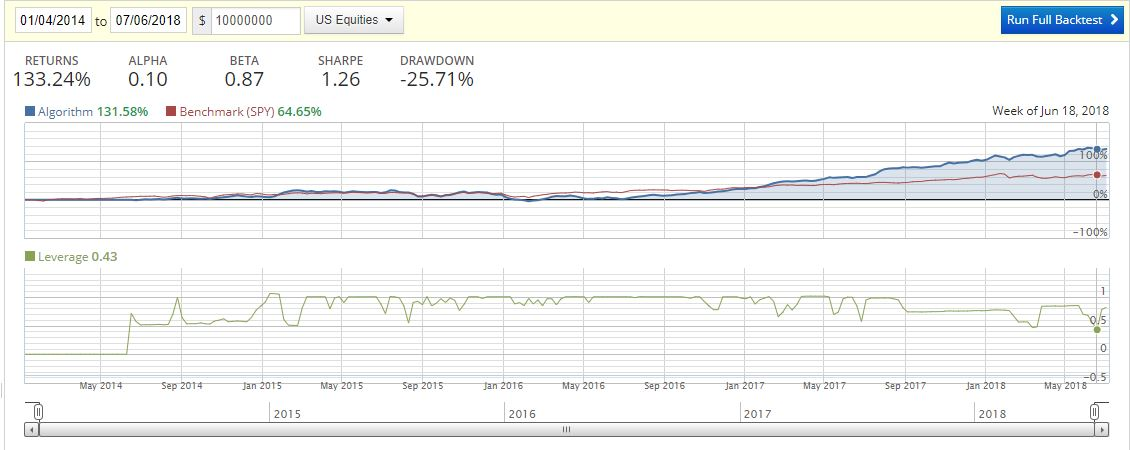
\includegraphics{img/Machine_Learning_1.png}
\caption{Algorithm 1 Result}
\end{figure}

    \subsubsection{Algorithm 2}\label{algorithm-2}

    \begin{itemize}
\tightlist
\item
  In this algorithm, I used simple moving average SMA and momentum
  indicators ADX, RSI to predict the next movement.
\item
  The stocks to take is chosen by volume with percentile from 99.5 to
  100.
\item
  The algorithm predict if a stock will move up or not.
\item
  A bagging of three classifiers were employed in the prediction, which
  are Adaboost and GaussianNB
\item
  The strategy longs stock if the stock is predicted up and cashes out
  otherwise.
\end{itemize}

    \begin{Verbatim}[commandchars=\\\{\}]
{\color{incolor}In [{\color{incolor} }]:} \PY{k+kn}{from} \PY{n+nn}{talib} \PY{k}{import} \PY{n}{SMA}\PY{p}{,} \PY{n}{ADX}\PY{p}{,} \PY{n}{RSI}
        \PY{k+kn}{import} \PY{n+nn}{numpy} \PY{k}{as} \PY{n+nn}{np}
        \PY{k+kn}{from} \PY{n+nn}{sklearn}\PY{n+nn}{.}\PY{n+nn}{naive\PYZus{}bayes} \PY{k}{import} \PY{n}{GaussianNB}
        \PY{k+kn}{from} \PY{n+nn}{sklearn}\PY{n+nn}{.}\PY{n+nn}{ensemble} \PY{k}{import} \PY{n}{AdaBoostClassifier} \PY{k}{as} \PY{n}{Adaboost}
        
        \PY{k}{def} \PY{n+nf}{initialize}\PY{p}{(}\PY{n}{context}\PY{p}{)}\PY{p}{:}
            
            \PY{c+c1}{\PYZsh{}Variables to change    }
            \PY{n}{context}\PY{o}{.}\PY{n}{lookback} \PY{o}{=} \PY{l+m+mi}{1250}          \PY{c+c1}{\PYZsh{}How many bars of data to use in the machine learning classifier}
            \PY{n}{context}\PY{o}{.}\PY{n}{omit} \PY{o}{=} \PY{l+m+mi}{251}               \PY{c+c1}{\PYZsh{}How many points to omit.  To get rid of nan\PYZsq{}s.  Currently set to 251 for the 250 day SMA}
            \PY{n}{context}\PY{o}{.}\PY{n}{timeframe} \PY{o}{=} \PY{l+m+mi}{20}           \PY{c+c1}{\PYZsh{}How often are we trading? Weekly? 5.  Monthly? 20.}
            \PY{n}{context}\PY{o}{.}\PY{n}{time\PYZus{}to\PYZus{}run} \PY{o}{=} \PY{l+m+mi}{15}         \PY{c+c1}{\PYZsh{}How many minutes before market close to trade}
            \PY{n}{context}\PY{o}{.}\PY{n}{gain\PYZus{}cutoff} \PY{o}{=} \PY{l+m+mf}{0.01}       \PY{c+c1}{\PYZsh{}What percent gain is needs to be predicted before going long}
            \PY{n}{context}\PY{o}{.}\PY{n}{target\PYZus{}levervage} \PY{o}{=} \PY{l+m+mf}{1.0}   \PY{c+c1}{\PYZsh{}Target leverage}
            \PY{n}{context}\PY{o}{.}\PY{n}{ML}\PY{o}{=}\PY{n}{ML\PYZus{}classifiers}\PY{p}{(} \PY{p}{[}\PY{n}{Adaboost}\PY{p}{(}\PY{p}{)}\PY{p}{,}  \PY{n}{GaussianNB}\PY{p}{(}\PY{p}{)}\PY{p}{]}\PY{p}{)} \PY{c+c1}{\PYZsh{}bagging classifier of two    }
            \PY{c+c1}{\PYZsh{}Stocks to trade}
            \PY{n}{set\PYZus{}universe}\PY{p}{(}\PY{n}{universe}\PY{o}{.}\PY{n}{DollarVolumeUniverse}\PY{p}{(}\PY{n}{floor\PYZus{}percentile}\PY{o}{=}\PY{l+m+mf}{99.5}\PY{p}{,} \PY{n}{ceiling\PYZus{}percentile}\PY{o}{=}\PY{l+m+mi}{100}\PY{p}{)}\PY{p}{)} 
            
            \PY{n}{schedule\PYZus{}function}\PY{p}{(}\PY{n}{rebalance}\PY{p}{,} \PY{n}{date\PYZus{}rules}\PY{o}{.}\PY{n}{month\PYZus{}start}\PY{p}{(}\PY{p}{)}\PY{p}{,} \PY{n}{time\PYZus{}rules}\PY{o}{.}\PY{n}{market\PYZus{}close}\PY{p}{(}\PY{n}{minutes}\PY{o}{=}\PY{p}{(}\PY{n}{context}\PY{o}{.}\PY{n}{time\PYZus{}to\PYZus{}run}\PY{o}{+}\PY{l+m+mi}{2}\PY{p}{)}\PY{p}{)}\PY{p}{,} \PY{n}{half\PYZus{}days}\PY{o}{=}\PY{k+kc}{True}\PY{p}{)}  \PY{c+c1}{\PYZsh{}Get the data}
        
            
        
        \PY{k}{def} \PY{n+nf}{handle\PYZus{}data}\PY{p}{(}\PY{n}{context}\PY{p}{,} \PY{n}{data}\PY{p}{)}\PY{p}{:}
            \PY{n}{record}\PY{p}{(}\PY{n}{leverage}\PY{o}{=}\PY{n}{context}\PY{o}{.}\PY{n}{account}\PY{o}{.}\PY{n}{leverage}\PY{p}{)}
            
        \PY{c+c1}{\PYZsh{}Getting the data, formatting the features and labels.}
        \PY{k}{def} \PY{n+nf}{rebalance}\PY{p}{(}\PY{n}{context}\PY{p}{,} \PY{n}{data}\PY{p}{)}\PY{p}{:}
            
            \PY{c+c1}{\PYZsh{}Pricing data}
            \PY{n}{prices} \PY{o}{=} \PY{n}{history}\PY{p}{(}\PY{n}{context}\PY{o}{.}\PY{n}{lookback}\PY{p}{,} \PY{l+s+s1}{\PYZsq{}}\PY{l+s+s1}{1d}\PY{l+s+s1}{\PYZsq{}}\PY{p}{,} \PY{l+s+s1}{\PYZsq{}}\PY{l+s+s1}{price}\PY{l+s+s1}{\PYZsq{}}\PY{p}{)}
            \PY{n}{highs} \PY{o}{=} \PY{n}{history}\PY{p}{(}\PY{n}{context}\PY{o}{.}\PY{n}{lookback}\PY{p}{,} \PY{l+s+s1}{\PYZsq{}}\PY{l+s+s1}{1d}\PY{l+s+s1}{\PYZsq{}}\PY{p}{,} \PY{l+s+s1}{\PYZsq{}}\PY{l+s+s1}{high}\PY{l+s+s1}{\PYZsq{}}\PY{p}{)}
            \PY{n}{lows} \PY{o}{=} \PY{n}{history}\PY{p}{(}\PY{n}{context}\PY{o}{.}\PY{n}{lookback}\PY{p}{,} \PY{l+s+s1}{\PYZsq{}}\PY{l+s+s1}{1d}\PY{l+s+s1}{\PYZsq{}}\PY{p}{,} \PY{l+s+s1}{\PYZsq{}}\PY{l+s+s1}{low}\PY{l+s+s1}{\PYZsq{}}\PY{p}{)}
        
            
            \PY{c+c1}{\PYZsh{}Clear the lists so that some points are not repeated}
            \PY{n}{hold\PYZus{}list} \PY{o}{=} \PY{p}{[}\PY{p}{]}           \PY{c+c1}{\PYZsh{} holding list of stocks}
            \PY{n}{feature\PYZus{}test}\PY{o}{=}\PY{p}{\PYZob{}}\PY{p}{\PYZcb{}}          \PY{c+c1}{\PYZsh{} features to predict, indexed by stock}
            \PY{n}{X}\PY{p}{,}\PY{n}{y}\PY{o}{=}\PY{p}{[}\PY{p}{]}\PY{p}{,}\PY{p}{[}\PY{p}{]}                \PY{c+c1}{\PYZsh{} list holds features and label}
            \PY{k}{for} \PY{n}{stock} \PY{o+ow}{in} \PY{n}{data}\PY{p}{:}        
                \PY{c+c1}{\PYZsh{}Indicators simple moving average SMA and momentum indicators ADX, RSI }
                \PY{n}{feature\PYZus{}list}\PY{o}{=}\PY{p}{[}\PY{p}{]}
                \PY{n}{feature\PYZus{}list}\PY{o}{+}\PY{o}{=}\PY{n+nb}{list}\PY{p}{(}\PY{n+nb}{map}\PY{p}{(}\PY{k}{lambda}  \PY{n}{period} \PY{p}{:} \PY{n}{SMA}\PY{p}{(}\PY{n}{prices}\PY{p}{[}\PY{n}{stock}\PY{p}{]}\PY{p}{,} \PY{n}{timeperiod}\PY{o}{=}\PY{n}{period}\PY{p}{)}\PY{o}{/}\PY{n}{prices}\PY{p}{[}\PY{n}{stock}\PY{p}{]}\PY{p}{,} \PY{p}{[}\PY{l+m+mi}{5}\PY{p}{,}\PY{l+m+mi}{10}\PY{p}{,}\PY{l+m+mi}{20}\PY{p}{,}\PY{l+m+mi}{50}\PY{p}{,}\PY{l+m+mi}{100}\PY{p}{,}\PY{l+m+mi}{200}\PY{p}{,}\PY{l+m+mi}{250}\PY{p}{]}\PY{p}{)}\PY{p}{)}
                \PY{n}{feature\PYZus{}list}\PY{o}{+}\PY{o}{=}\PY{n+nb}{list}\PY{p}{(}\PY{n+nb}{map}\PY{p}{(}\PY{k}{lambda}  \PY{n}{period} \PY{p}{:} \PY{n}{ADX}\PY{p}{(}\PY{n}{highs}\PY{p}{[}\PY{n}{stock}\PY{p}{]}\PY{p}{,} \PY{n}{lows}\PY{p}{[}\PY{n}{stock}\PY{p}{]}\PY{p}{,}\PY{n}{prices}\PY{p}{[}\PY{n}{stock}\PY{p}{]}\PY{p}{,} \PY{n}{timeperiod}\PY{o}{=}\PY{n}{period}\PY{p}{)}\PY{o}{/}\PY{n}{prices}\PY{p}{[}\PY{n}{stock}\PY{p}{]}\PY{p}{,} \PY{p}{[}\PY{l+m+mi}{7}\PY{p}{,}\PY{l+m+mi}{14}\PY{p}{,}\PY{l+m+mi}{25}\PY{p}{]}\PY{p}{)}\PY{p}{)}
                \PY{n}{feature\PYZus{}list}\PY{o}{+}\PY{o}{=}\PY{n+nb}{list}\PY{p}{(}\PY{n+nb}{map}\PY{p}{(}\PY{k}{lambda}  \PY{n}{period} \PY{p}{:} \PY{n}{RSI}\PY{p}{(}\PY{n}{prices}\PY{p}{[}\PY{n}{stock}\PY{p}{]}\PY{p}{,} \PY{n}{timeperiod}\PY{o}{=}\PY{n}{period}\PY{p}{)}\PY{o}{/}\PY{n}{prices}\PY{p}{[}\PY{n}{stock}\PY{p}{]}\PY{p}{,} \PY{p}{[}\PY{l+m+mi}{7}\PY{p}{,}\PY{l+m+mi}{14}\PY{p}{,}\PY{l+m+mi}{25}\PY{p}{]}\PY{p}{)}\PY{p}{)}   
                
                \PY{c+c1}{\PYZsh{}Labels 1 means move up    }
                \PY{n}{labels}\PY{o}{=}\PY{p}{(}\PY{n}{prices}\PY{p}{[}\PY{n}{stock}\PY{p}{]}\PY{o}{.}\PY{n}{pct\PYZus{}change}\PY{p}{(}\PY{n}{periods}\PY{o}{=}\PY{n}{context}\PY{o}{.}\PY{n}{timeframe}\PY{p}{)}\PY{o}{\PYZgt{}}\PY{n}{context}\PY{o}{.}\PY{n}{gain\PYZus{}cutoff}\PY{p}{)}\PY{o}{.}\PY{n}{astype}\PY{p}{(}\PY{l+s+s1}{\PYZsq{}}\PY{l+s+s1}{int32}\PY{l+s+s1}{\PYZsq{}}\PY{p}{)}\PY{o}{.}\PY{n}{shift}\PY{p}{(}\PY{o}{\PYZhy{}}\PY{n}{context}\PY{o}{.}\PY{n}{timeframe}\PY{p}{)}\PY{c+c1}{\PYZsh{}The percent change of the stock represented as 5.46\PYZpc{}, \PYZhy{}13.2\PYZpc{} for example}
             
                \PY{c+c1}{\PYZsh{}Only go through the none nan values      }
                \PY{k}{for} \PY{n}{i} \PY{o+ow}{in} \PY{n+nb}{range}\PY{p}{(}\PY{n}{context}\PY{o}{.}\PY{n}{omit}\PY{p}{,} \PY{p}{(}\PY{n}{context}\PY{o}{.}\PY{n}{lookback}\PY{o}{\PYZhy{}}\PY{n}{context}\PY{o}{.}\PY{n}{timeframe}\PY{p}{)}\PY{p}{)}\PY{p}{:}
                    \PY{c+c1}{\PYZsh{}collect features by date       }
                    \PY{n}{features}\PY{o}{=}\PY{p}{[} \PY{n}{item}\PY{p}{[}\PY{n}{i}\PY{p}{]}  \PY{k}{for} \PY{n}{item} \PY{o+ow}{in} \PY{n}{feature\PYZus{}list}\PY{p}{]} 
                     \PY{c+c1}{\PYZsh{}Check any nan value in the features   }
                    \PY{k}{if} \PY{o+ow}{not} \PY{n}{np}\PY{o}{.}\PY{n}{isnan}\PY{p}{(}\PY{n}{features}\PY{p}{)}\PY{o}{.}\PY{n}{any}\PY{p}{(}\PY{p}{)}\PY{p}{:}             
                        \PY{n}{X}\PY{o}{.}\PY{n}{append}\PY{p}{(}\PY{n}{features}\PY{p}{)}             
                        \PY{n}{y}\PY{o}{.}\PY{n}{append}\PY{p}{(}\PY{n}{labels}\PY{p}{[}\PY{n}{i}\PY{p}{]}\PY{p}{)}
                       
                        
                \PY{c+c1}{\PYZsh{} gather feature to predict        }
                \PY{n}{tmp}\PY{o}{=}\PY{p}{[} \PY{n}{item}\PY{p}{[}\PY{o}{\PYZhy{}}\PY{l+m+mi}{1}\PY{p}{]}  \PY{k}{for} \PY{n}{item} \PY{o+ow}{in} \PY{n}{feature\PYZus{}list}\PY{p}{]}
                \PY{k}{if} \PY{o+ow}{not} \PY{n}{np}\PY{o}{.}\PY{n}{isnan}\PY{p}{(}\PY{n}{tmp}\PY{p}{)}\PY{o}{.}\PY{n}{any}\PY{p}{(}\PY{p}{)}\PY{p}{:}
                    \PY{n}{feature\PYZus{}test}\PY{p}{[}\PY{n}{stock}\PY{p}{]}\PY{o}{=}\PY{n}{tmp}
                    
                    
            \PY{c+c1}{\PYZsh{} train model        }
            \PY{n}{context}\PY{o}{.}\PY{n}{ML}\PY{o}{.}\PY{n}{fit}\PY{p}{(}\PY{n}{X}\PY{p}{,}\PY{n}{y}\PY{p}{)}
            \PY{k}{for} \PY{n}{stock} \PY{o+ow}{in} \PY{n}{data}\PY{p}{:}
                \PY{k}{if} \PY{n}{stock} \PY{o+ow}{in} \PY{n}{feature\PYZus{}test} \PY{p}{:}
                    \PY{c+c1}{\PYZsh{} predict by sum of predictions}
                    \PY{n}{predict}\PY{o}{=}\PY{n+nb}{sum}\PY{p}{(}\PY{n}{context}\PY{o}{.}\PY{n}{ML}\PY{o}{.}\PY{n}{predict}\PY{p}{(}\PY{n}{feature\PYZus{}test}\PY{p}{[}\PY{n}{stock}\PY{p}{]}\PY{p}{)}\PY{p}{)}
                    \PY{c+c1}{\PYZsh{} if predicted move up, add stock to holding list}
                    \PY{k}{if} \PY{n}{predict}\PY{o}{\PYZgt{}}\PY{l+m+mf}{1.5}\PY{p}{:}
                        \PY{n}{hold\PYZus{}list}\PY{o}{.}\PY{n}{append}\PY{p}{(}\PY{n}{stock}\PY{p}{)}
        
            \PY{c+c1}{\PYZsh{} calcualte weight according to holding list            }
            \PY{n}{weight}\PY{o}{=} \PY{n+nb}{float}\PY{p}{(}\PY{n}{context}\PY{o}{.}\PY{n}{target\PYZus{}levervage} \PY{o}{/} \PY{n+nb}{len}\PY{p}{(}\PY{n}{hold\PYZus{}list}\PY{p}{)}\PY{p}{)} \PY{k}{if} \PY{n}{hold\PYZus{}list} \PY{k}{else} \PY{l+m+mf}{0.0}
            \PY{c+c1}{\PYZsh{} Make orders}
            \PY{k}{for} \PY{n}{stock} \PY{o+ow}{in} \PY{n}{data}\PY{p}{:}
                \PY{k}{if} \PY{n}{stock} \PY{o+ow}{in} \PY{n}{hold\PYZus{}list}\PY{p}{:}
                    \PY{n}{order\PYZus{}target\PYZus{}percent}\PY{p}{(}\PY{n}{stock}\PY{p}{,} \PY{n}{weight}\PY{p}{)}
                \PY{k}{else}\PY{p}{:} 
                    \PY{n}{order\PYZus{}target\PYZus{}percent}\PY{p}{(}\PY{n}{stock}\PY{p}{,} \PY{l+m+mf}{0.0}\PY{p}{)}  
\end{Verbatim}


    \textbf{Backtest Result}

    \begin{figure}
\centering
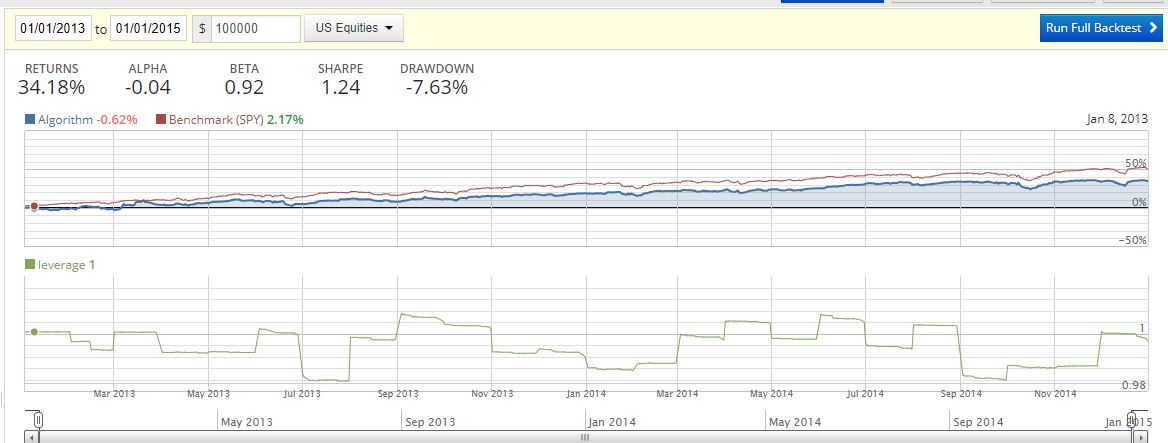
\includegraphics{img/Machine_Learning_2.png}
\caption{Algorithm 2 Result}
\end{figure}


    % Add a bibliography block to the postdoc
    
    
    
    \end{document}
